\documentclass[11pt,a4paper]{article}

% % Fonts and encoding
% \usepackage[utf8]{inputenc}
% \usepackage[T1]{fontenc}
% \usepackage[english]{babel}

% Usual packages
\usepackage{amsmath}
\usepackage{graphicx}
\usepackage[hidelinks=true]{hyperref}
\usepackage[margin=2.5cm]{geometry}
\usepackage{booktabs}
\usepackage{array}
\usepackage{float}
\newcommand{\bm}{\mathbf}

% Font
\usepackage{cmbright}

% SI units
\usepackage{siunitx}

% References
\usepackage{cleveref}

\title{\textbf{AERO70016 Orbital Mechanics Coursework 2025--26}\\[4pt]
\large AURORA Mission: Special Perturbations and Ground Station Analysis}
\author{Himmat Kaul \\ CID: 02376386}
\date{20th March 2026}

\begin{document}
\maketitle

% ─────────────────────────────────────────────────────────────
\section*{Part (a): One-Year Orbit Propagation with Perturbations}
% ─────────────────────────────────────────────────────────────

\subsection*{(a.i) Numerical Method}

The AURORA orbit is propagated using \textbf{Cowell's method} (special perturbations), which integrates the equations of motion directly in Cartesian ECI coordinates:
\begin{equation}
    \ddot{\bm{r}} = -\frac{\mu}{r^3}\bm{r} + \bm{a}_{J2} + \bm{a}_{\mathrm{drag}} + \bm{a}_{\mathrm{SRP}} + \bm{a}_{\mathrm{lsol}},
    \label{eq:eom}
\end{equation}
where $\mu = \SI{3.9860e14}{m^3 s^{-2}}$ is Earth's gravitational parameter and $r = \|\bm{r}\|$.

The integrator chosen is \textbf{DOP853} (8th-order Dormand--Prince explicit Runge--Kutta), implemented via \texttt{scipy.integrate.solve\_ivp}. This method is well-suited to orbital propagation for several reasons. Its high order (8) achieves excellent accuracy per function evaluation, which is critical for a year-long integration with tight tolerances. Local error control is applied with relative tolerance $\varepsilon_r = 10^{-10}$ and absolute tolerance $\varepsilon_a = 10^{-12}$\,m (position) and $10^{-12}$\,m\,s$^{-1}$ (velocity), ensuring energy errors remain below $10^{-9}$ relative over the full year. A maximum step size of \SI{300}{s} is imposed to prevent the integrator from stepping over the perigee passage, where the gravitational and drag accelerations change rapidly. Output is evaluated hourly for orbital element analysis.

The state vector is $\bm{X} = [\bm{r},\,\bm{v}]^T \in \mathbb{R}^6$, and Keplerian elements $\{a, e, i, \Omega, \omega, \nu\}$ are recovered from each output state using the standard orbital mechanics relations.

\subsection*{(a.ii) Perturbations Included}

Four perturbations are included in the force model. Their selection is justified by comparing acceleration magnitudes over one orbital period, shown in \cref{fig:perturb_comparison}.

\begin{figure}[H]
    \centering
    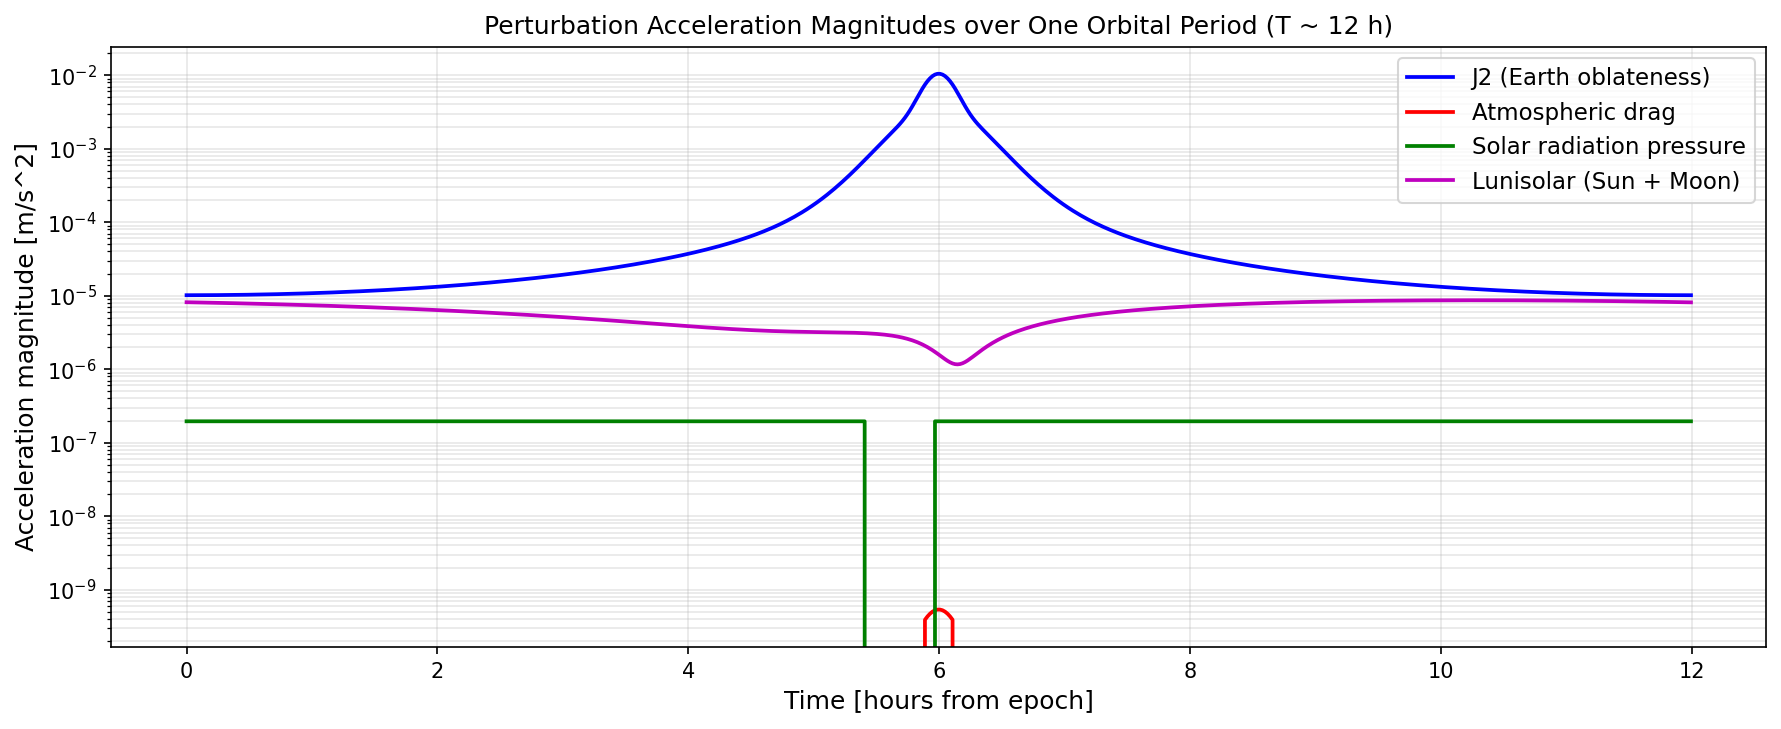
\includegraphics[width=0.92\textwidth]{figs/partA_perturbation_comparison.png}
    \caption{Perturbation acceleration magnitudes over one orbital period (T $\approx$ \SI{12}{h}). The step change in drag at perigee passage is clearly visible.\label{fig:perturb_comparison}}
\end{figure}

\paragraph{J2 (Earth oblateness).} The leading non-spherical harmonic, with coefficient $J_2 = 1.0826 \times 10^{-3}$. The resulting acceleration is:
\begin{equation}
    \bm{a}_{J2} = -\frac{3}{2}\frac{\mu J_2 R_E^2}{r^5}\left[\left(1 - 5\left(\frac{z}{r}\right)^2\right)(x\hat{\bm{e}}_x + y\hat{\bm{e}}_y) + \left(3 - 5\left(\frac{z}{r}\right)^2\right)z\hat{\bm{e}}_z\right].
\end{equation}
At perigee ($r_p \approx \SI{7980}{km}$, altitude \SI{1602}{km}), $|\bm{a}_{J2}| \approx 1.04\times10^{-2}$\,m\,s$^{-2}$, exceeding all other perturbations by several orders of magnitude. At apogee ($r_a \approx \SI{45220}{km}$), it falls to $1.01\times10^{-5}$\,m\,s$^{-2}$ but remains the dominant perturbation. Higher harmonics ($J_3$, $J_4$, \ldots) are smaller by at least two orders of magnitude and are neglected.

\paragraph{Atmospheric drag.} Significant only at low altitudes. The drag acceleration is:
\begin{equation}
    \bm{a}_{\mathrm{drag}} = -\frac{1}{2}C_D\frac{A}{m}\rho\,v_{\mathrm{rel}}^2\,\hat{\bm{v}}_{\mathrm{rel}},
\end{equation}
with $C_D = 2.2$, $A/m = 20/700$\,m$^2$\,kg$^{-1}$, and density $\rho$ from a layered exponential atmosphere. The velocity is taken relative to the co-rotating atmosphere. At the perigee altitude of \SI{1602}{km}, $\rho \approx 1.9\times10^{-16}$\,kg\,m$^{-3}$, giving $|\bm{a}_{\mathrm{drag}}| \approx 5.4\times10^{-10}$\,m\,s$^{-2}$ — seven orders of magnitude below J2. Drag is set to zero above \SI{2000}{km} and plays a negligible role at this perigee altitude.

\paragraph{Solar radiation pressure (SRP).} Acts at all altitudes outside Earth's cylindrical shadow. The acceleration is:
\begin{equation}
    \bm{a}_{\mathrm{SRP}} = \nu C_R \frac{A}{m} P_\odot \left(\frac{1\,\mathrm{AU}}{r_\odot}\right)^2 \hat{\bm{r}}_{\odot},
\end{equation}
where $P_\odot = \SI{4.56e-6}{N m^{-2}}$, $C_R = 1.5$, and $\nu \in \{0,1\}$ is the eclipse indicator. SRP is approximately constant over the orbit at $|\bm{a}_{\mathrm{SRP}}| \approx 1.95\times10^{-7}$\,m\,s$^{-2}$, consistent with the large $A/m$ ratio.

\paragraph{Lunisolar third-body perturbations.} The Sun and Moon introduce tidal perturbations via:
\begin{equation}
    \bm{a}_{\mathrm{lsol}} = \mu_\odot\left(\frac{\bm{r}_\odot - \bm{r}}{|\bm{r}_\odot - \bm{r}|^3} - \frac{\bm{r}_\odot}{r_\odot^3}\right) + \mu_\mathcal{L}\left(\frac{\bm{r}_\mathcal{L} - \bm{r}}{|\bm{r}_\mathcal{L} - \bm{r}|^3} - \frac{\bm{r}_\mathcal{L}}{r_\mathcal{L}^3}\right).
\end{equation}
At perigee, $|\bm{a}_{\mathrm{lsol}}| \approx 1.54\times10^{-6}$\,m\,s$^{-2}$; at apogee, $8.1\times10^{-6}$\,m\,s$^{-2}$ — making it the second-largest perturbation at high altitude, exceeding SRP by a factor of $\sim$40. Its long-period effect drives the eccentricity and inclination oscillations seen in Part (a.iii). Sun and Moon positions are computed from low-precision analytical series valid to $\sim$1\,arcmin (Meeus).

\subsection*{(a.iii) Qualitative Evolution of Orbital Elements}

\begin{figure}[H]
    \centering
    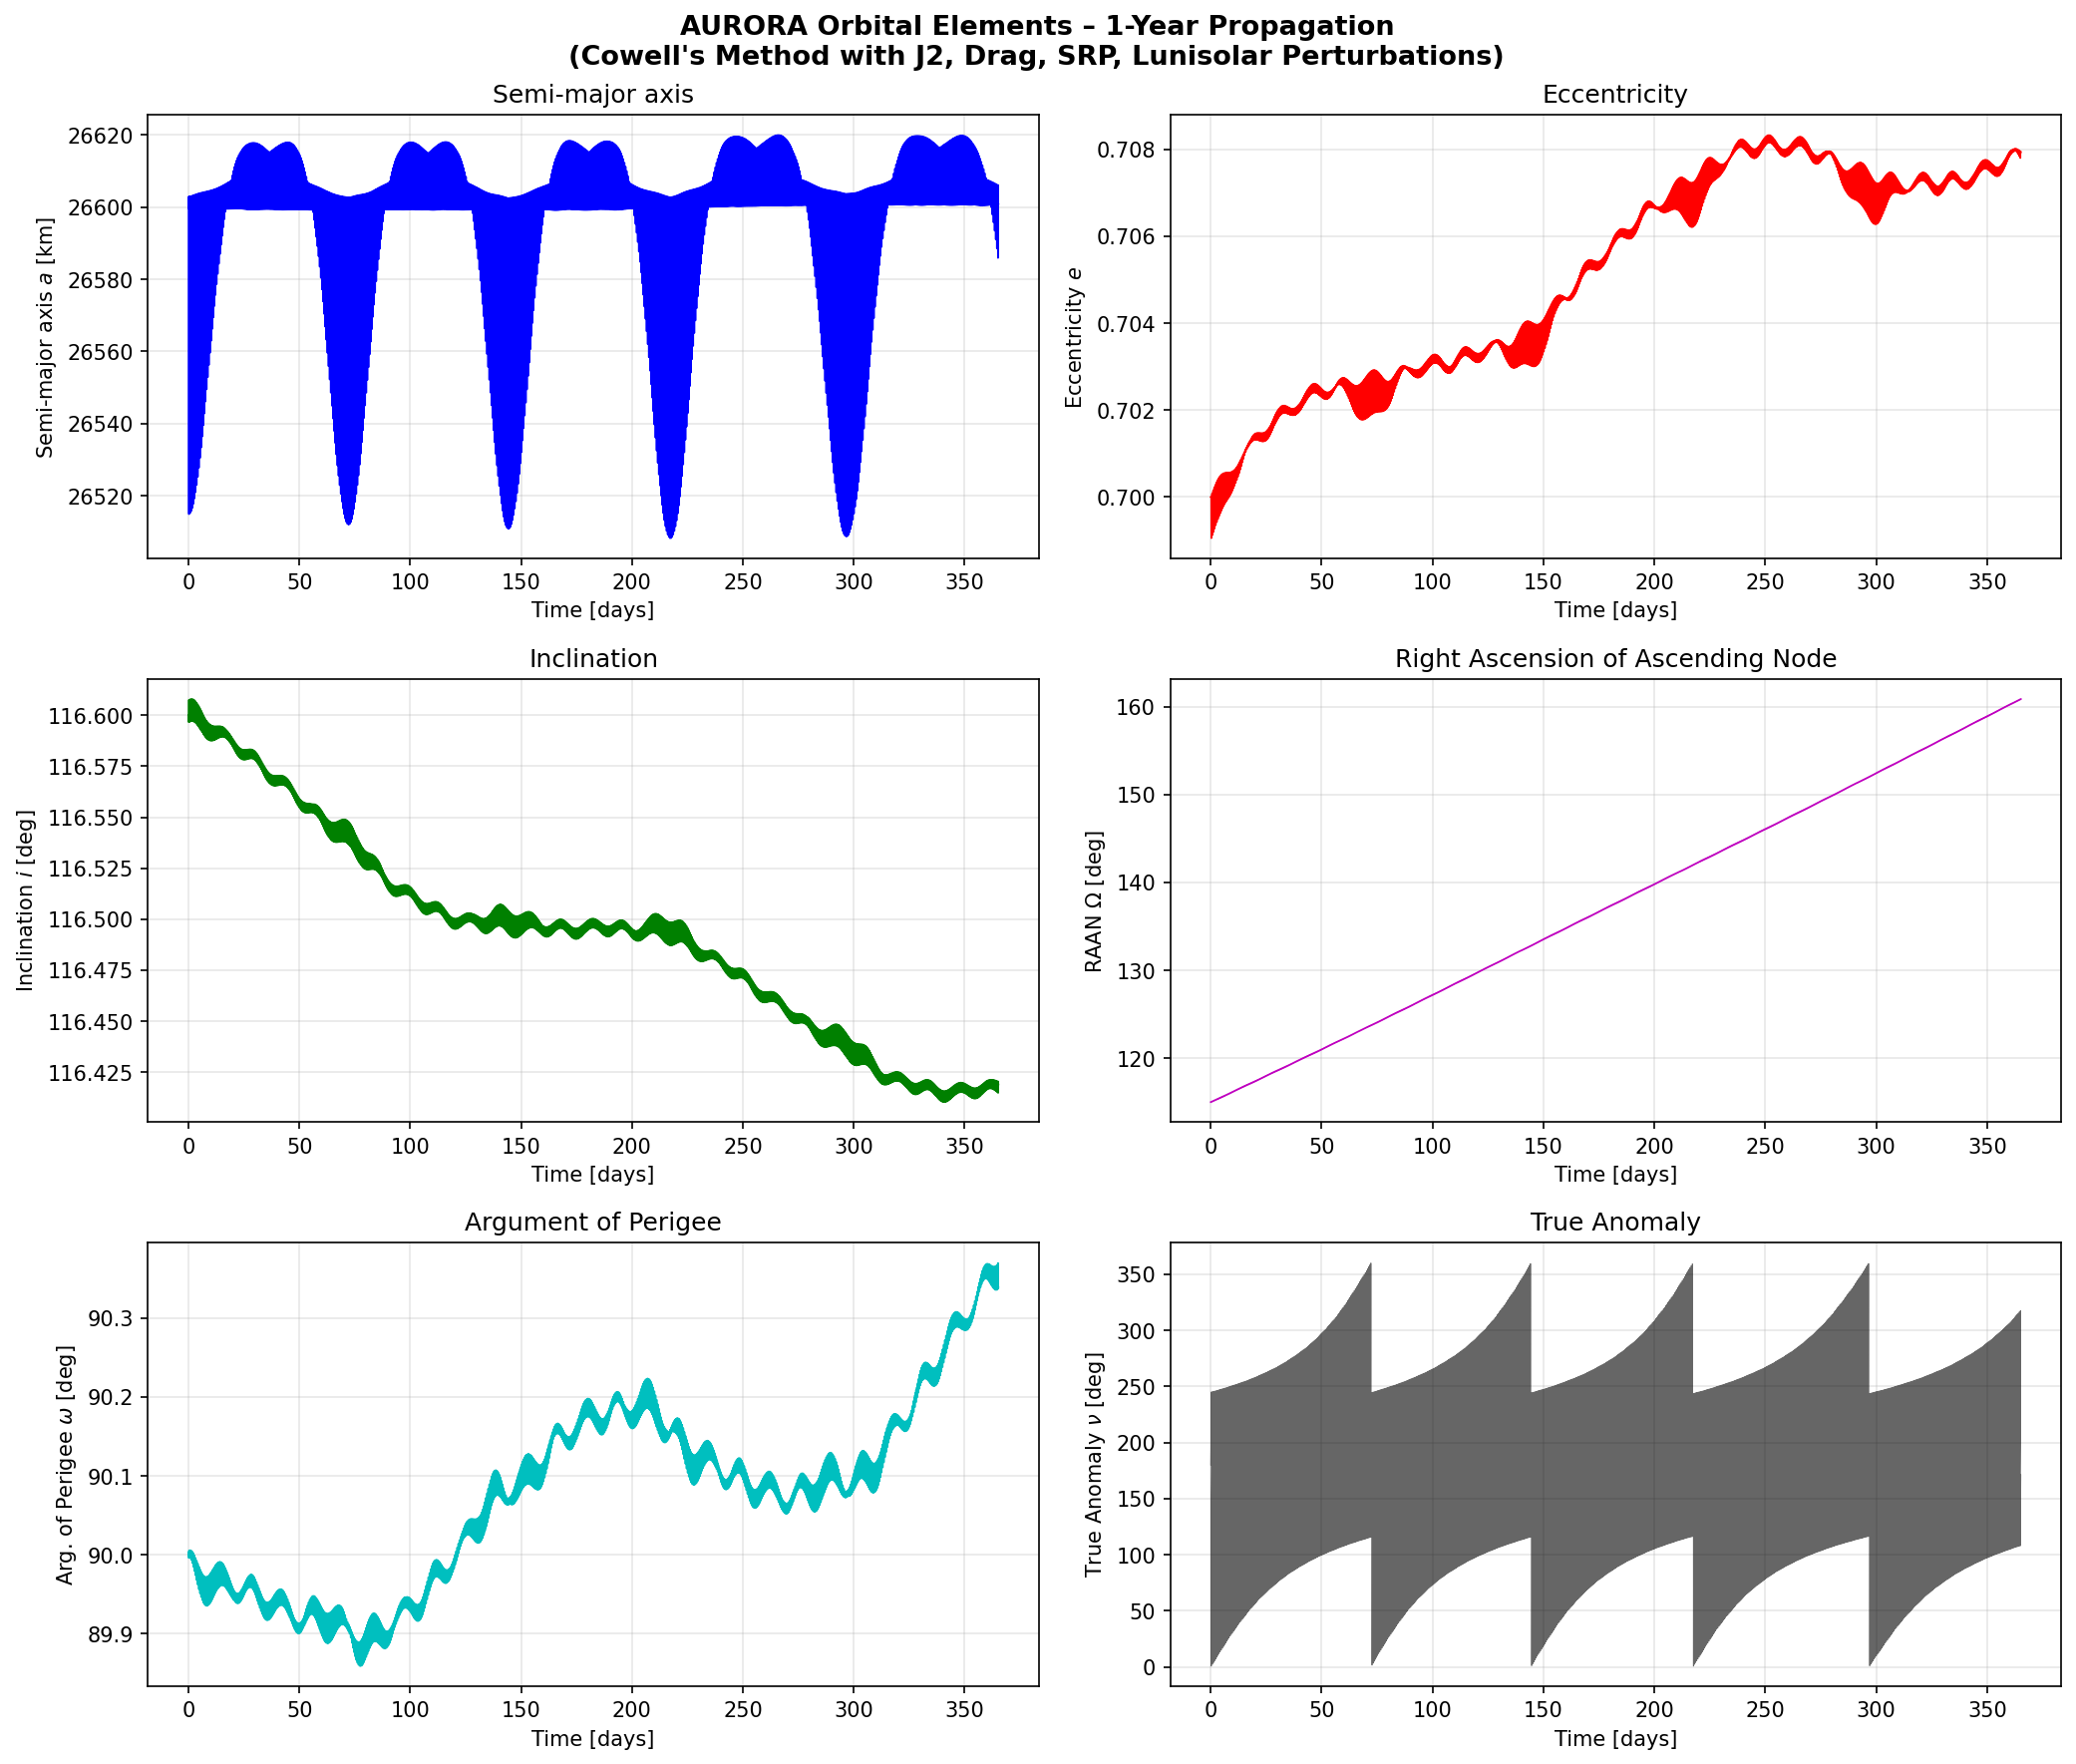
\includegraphics[width=\textwidth]{figs/partA_orbital_elements.png}
    \caption{Six orbital elements of AURORA over one year. The 1-hour output cadence resolves long-period trends while averaging over the short-period ($\sim$\SI{12}{h}) oscillations.\label{fig:orb_elems}}
\end{figure}

\begin{figure}[H]
    \centering
    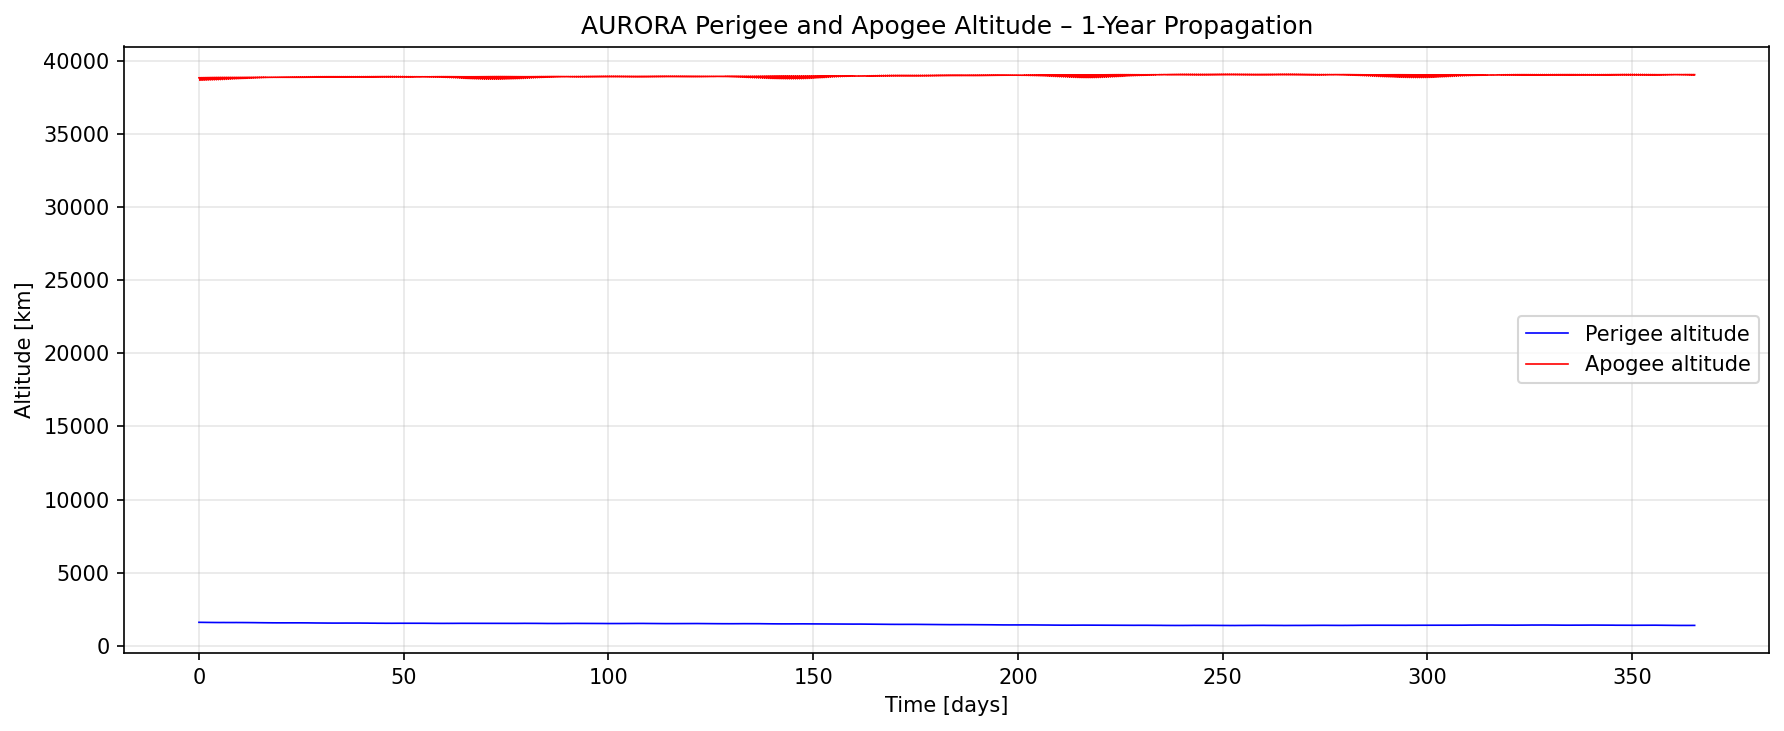
\includegraphics[width=0.85\textwidth]{figs/partA_altitude_history.png}
    \caption{Perigee and apogee altitude history over one year. The bounded oscillations confirm the orbit's long-term stability with negligible secular decay.\label{fig:alt_hist}}
\end{figure}

\paragraph{Semi-major axis $a$.}
Over one year, $a$ changes by $\Delta a \approx +\SI{0.77}{km}$ (from \SI{26600}{km}). The dominant driver is drag, which in principle removes energy and reduces $a$ (orbital decay). However, the drag acceleration is only $\sim 10^{-9}$\,m\,s$^{-2}$ at perigee — several orders of magnitude below J2 — and the high eccentricity means the spacecraft spends only a brief fraction of each 12-hour orbit in the denser lower atmosphere. Lunisolar perturbations pump energy into the orbit secularly, partially counteracting drag. The net result is a very small and slowly varying $a$. Short-period oscillations with amplitude $\sim\SI{10}{km}$ per orbit are visible, driven by J2 and the eccentric orbit geometry. No secular decay is evident at this scale.

\paragraph{Eccentricity $e$.}
The eccentricity shows $\Delta e \approx +0.008$ over the year, with prominent long-period ($\sim$90-day) oscillations superimposed on a small secular trend. These long-period variations are driven by lunisolar perturbations (primarily the Sun), which pump eccentricity through the Kozai--Lidov-type mechanism when the orbit's apogee aligns with the perturber. The short-period oscillations of $e$ are correlated with J2 and the orbit's changing orientation relative to Earth's equatorial bulge. Drag tends to circularise the orbit (reduce $e$), but its magnitude here is too small for a measurable secular effect over one year.

\paragraph{Inclination $i$.}
The inclination changes by $\Delta i \approx -0.18°$ over one year, exhibiting long-period oscillations at the same $\sim$90-day cadence as eccentricity (these are coupled through the Kozai mechanism). J2 alone causes no secular change in $i$; the residual drift is lunar and solar in origin. The short-period J2 oscillations in $i$ are below the 1-hour output resolution and average out.

\paragraph{RAAN $\Omega$.}
The right ascension of the ascending node drifts secularly at $\Delta\Omega \approx +45.9°$/year. The J2 secular formula is:
\begin{equation}
    \dot{\Omega} = -\frac{3}{2}n J_2 \left(\frac{R_E}{p}\right)^2 \cos i,
    \label{eq:raan_drift}
\end{equation}
where $p = a(1-e^2)$ is the semi-latus rectum and $n = \sqrt{\mu/a^3}$ is the mean motion. With $i = 116.6°$, $\cos i = -0.449$, so $\dot{\Omega} > 0$ (eastward drift), consistent with the prograde RAAN drift observed for retrograde orbits. The analytical estimate gives $\dot{\Omega} \approx +0.126$°/day $ = +45.9$°/year, in excellent agreement with the simulation. The slight non-linearity over the year reflects the coupling of RAAN drift with the evolving eccentricity.

\paragraph{Argument of perigee $\omega$.}
The argument of perigee shows near-zero secular drift ($\Delta\omega \approx +0.34°$/year) with large short-period oscillations. This is the defining characteristic of the \textbf{frozen orbit} (critical inclination). The J2 secular drift rate is:
\begin{equation}
    \dot{\omega} = \frac{3}{4}n J_2 \left(\frac{R_E}{p}\right)^2 (5\cos^2 i - 1).
    \label{eq:omega_drift}
\end{equation}
At $i = 116.6° = 180° - 63.4°$, we have $\cos^2 i = \cos^2(63.4°) = 0.200$, giving $5\cos^2 i - 1 = 0.0$. This is the retrograde critical inclination ($i_c = 180° - 63.435°$), for which $\dot{\omega} = 0$ secularly. The AURORA orbit thus maintains a stable apogee location, ensuring consistent coverage geometry over the mission lifetime. The residual drift of $+0.34$°/year is due to higher-order J2 terms and lunisolar perturbations.

% ─────────────────────────────────────────────────────────────
\section*{Part (b): Ground Station Pass Analysis}
% ─────────────────────────────────────────────────────────────

Elevation angles and pass tables are computed by numerically propagating the state from epoch (1 Jan 2026 12:00 UTC) for 72 hours at 30-second resolution (DOP853, same tolerances as Part a), then computing the elevation angle of the spacecraft from each ground station in the ENZ (East--North--Zenith) topocentric frame. A pass is defined as the interval during which the elevation exceeds the \SI{5}{°} mask. Results are filtered to the 48-hour window ending 3 Jan 2026 12:00 UTC.

\subsection*{(b.i) Pass Tables}

\cref{fig:elev} shows the elevation angle time series for both stations. \cref{fig:pass_dur} compares perturbed and Keplerian pass durations.

\begin{figure}[H]
    \centering
    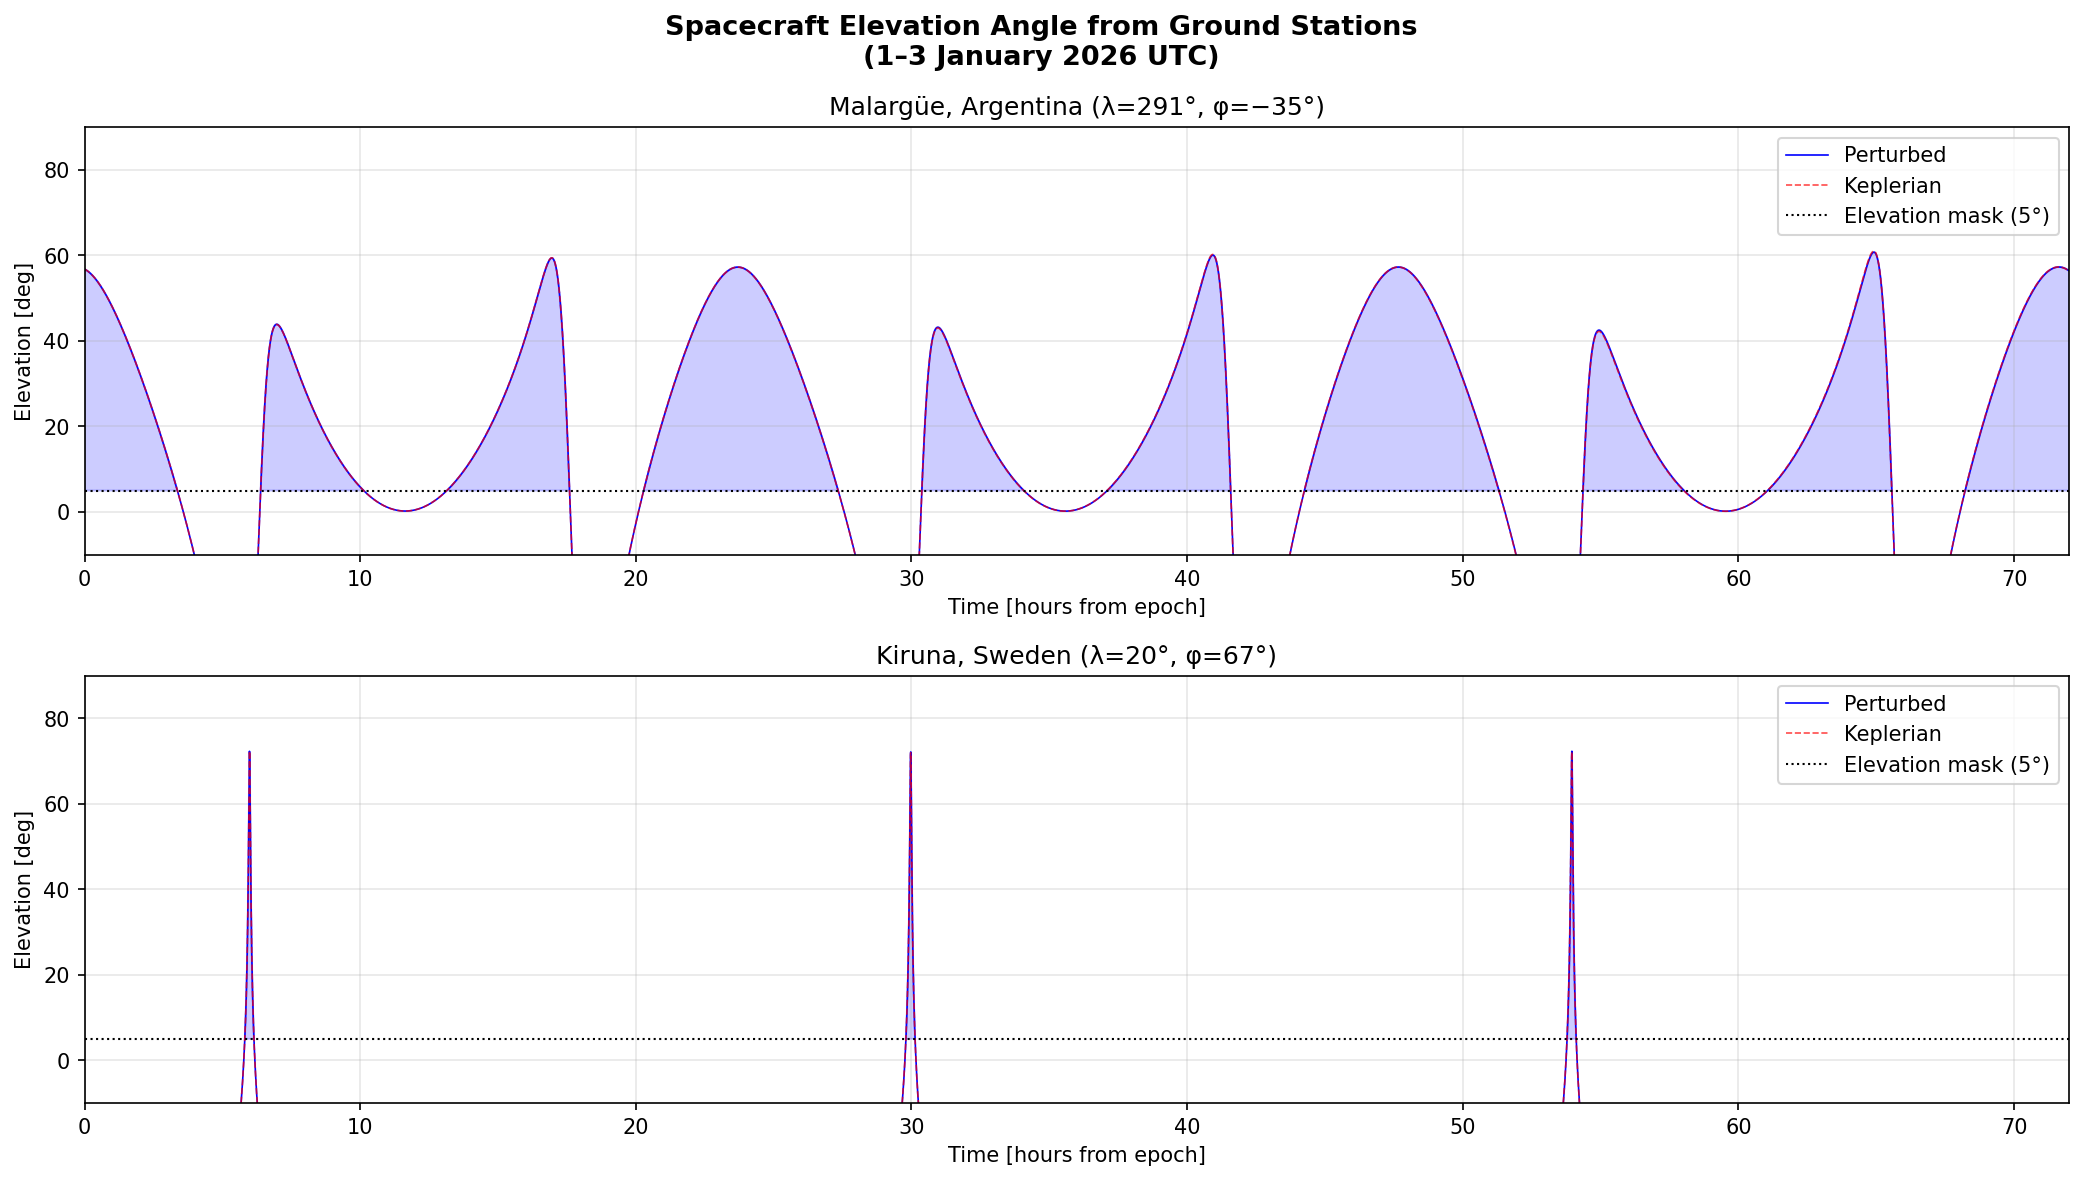
\includegraphics[width=\textwidth]{figs/partB_elevation_angles.png}
    \caption{Elevation angles of AURORA from Malarg\"{u}e (top) and Kiruna (bottom) over 72 hours from epoch. Blue: perturbed trajectory; red dashed: Keplerian. Shaded regions indicate visibility above the \SI{5}{°} elevation mask.\label{fig:elev}}
\end{figure}

\begin{figure}[H]
    \centering
    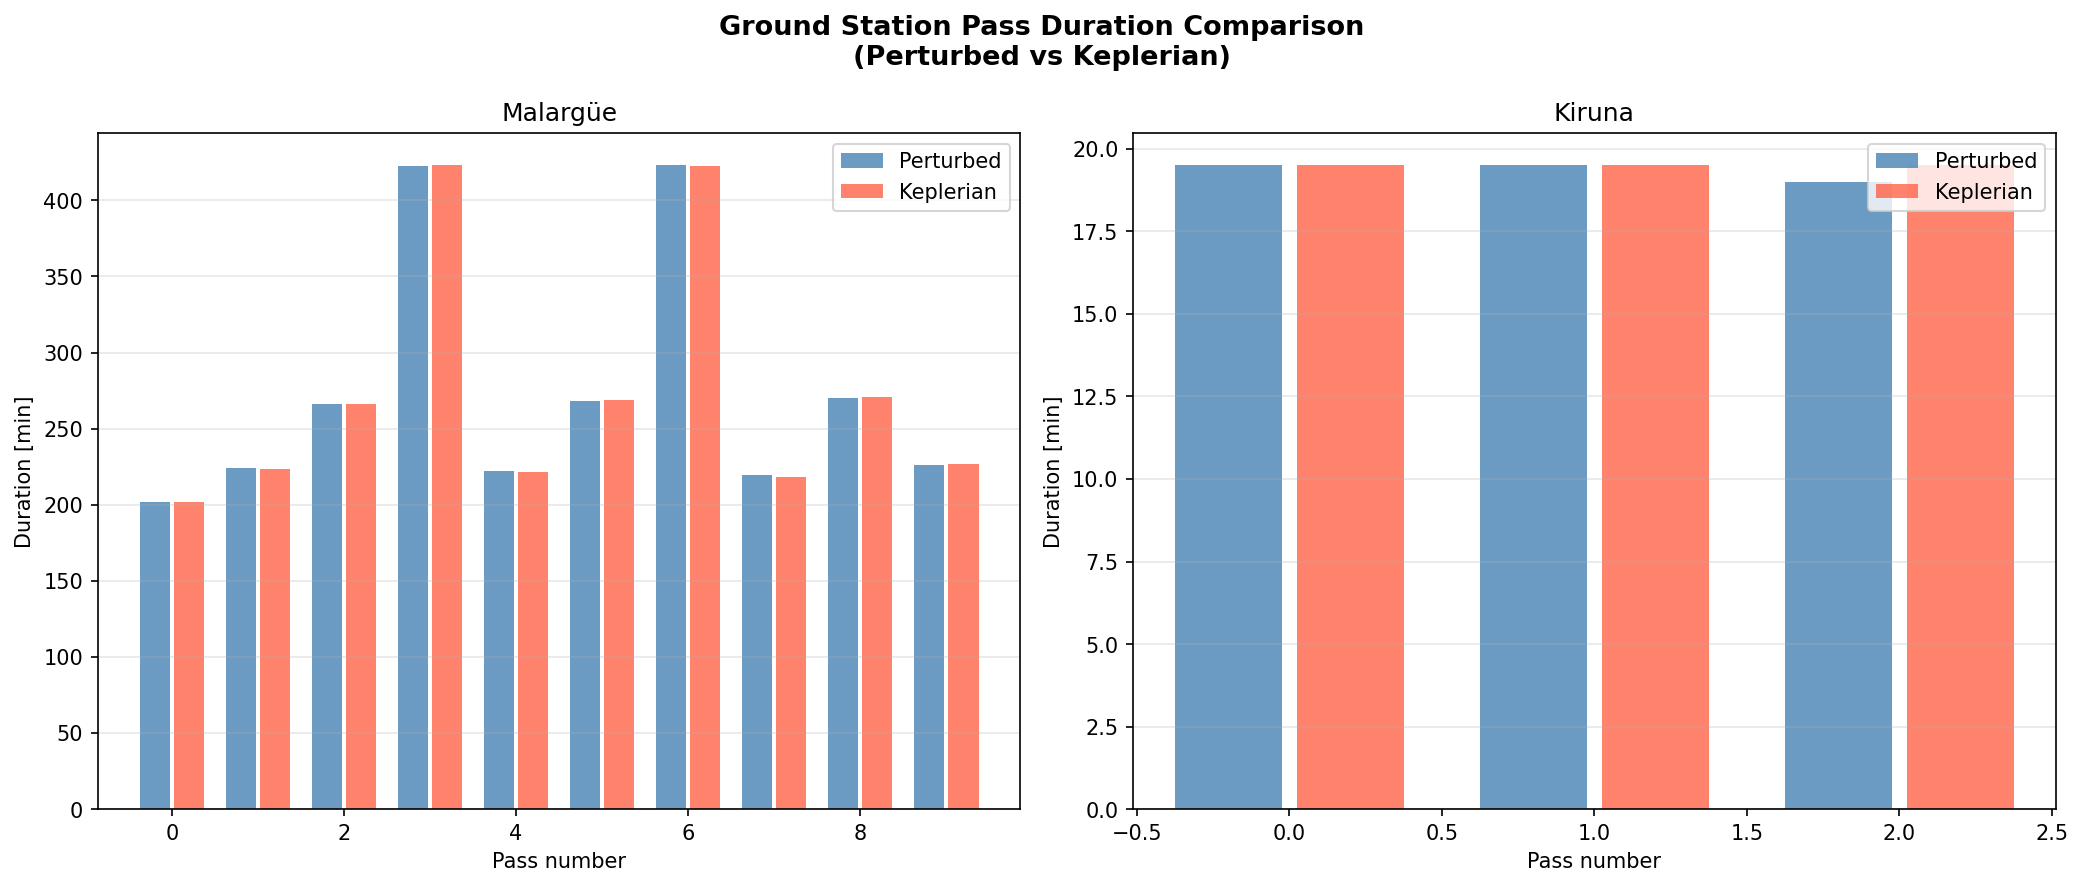
\includegraphics[width=0.85\textwidth]{figs/partB_pass_durations.png}
    \caption{Pass duration comparison between perturbed and Keplerian trajectories for Malarg\"{u}e and Kiruna over the 72-hour analysis window.\label{fig:pass_dur}}
\end{figure}

\begin{table}[H]
\centering
\caption{AURORA passes over \textbf{Malarg\"{u}e} ($\lambda=291°$, $\phi=-35°$) from 1--3 Jan 2026 UTC (48-hour window), perturbed trajectory. AOS = Acquisition of Signal; LOS = Loss of Signal.\label{tab:mal_p}}
\small
\begin{tabular}{@{}rllSS@{}}
\toprule
{Pass} & {AOS (UTC)} & {LOS (UTC)} & {Duration (min)} & {Max Elev. ($°$)} \\
\midrule
1 & 2026-01-01 12:00:00 & 2026-01-01 15:22:00 & 202.0 & 56.8 \\
2 & 2026-01-01 18:23:30 & 2026-01-01 22:07:30 & 224.0 & 43.9 \\
3 & 2026-01-02 01:09:00 & 2026-01-02 05:35:30 & 266.5 & 59.4 \\
4 & 2026-01-02 08:17:30 & 2026-01-02 15:20:00 & 422.5 & 57.3 \\
5 & 2026-01-02 18:22:30 & 2026-01-02 22:04:30 & 222.0 & 43.2 \\
6 & 2026-01-03 01:06:30 & 2026-01-03 05:34:30 & 268.0 & 60.1 \\
7 & 2026-01-03 08:15:30 & 2026-01-03 15:18:30 & 423.0 & 57.3 \\
\midrule
\multicolumn{3}{l}{\textit{Total contact time}} & 2028.0 & \\
\bottomrule
\end{tabular}
\end{table}

\begin{table}[H]
\centering
\caption{AURORA passes over \textbf{Kiruna} ($\lambda=20°$, $\phi=67°$) from 1--3 Jan 2026 UTC (48-hour window), perturbed trajectory.\label{tab:kir_p}}
\small
\begin{tabular}{@{}rllSS@{}}
\toprule
{Pass} & {AOS (UTC)} & {LOS (UTC)} & {Duration (min)} & {Max Elev. ($°$)} \\
\midrule
1 & 2026-01-01 17:49:00 & 2026-01-01 18:08:30 & 19.5 & 72.3 \\
2 & 2026-01-02 17:48:00 & 2026-01-02 18:07:30 & 19.5 & 72.1 \\
\midrule
\multicolumn{3}{l}{\textit{Total contact time}} & 39.0 & \\
\bottomrule
\end{tabular}
\end{table}

\subsection*{(b.ii) Comparison of Pass Durations}

The results reveal a striking asymmetry: Malarg\"{u}e accumulates \SI{2028}{min} of contact over 7 passes, while Kiruna achieves only \SI{39}{min} over 2 passes — a factor of $\sim$52$\times$ difference. This is explained by the orbital geometry.

The AURORA orbit has $a = \SI{26600}{km}$, $e = 0.7$, giving perigee \SI{1602}{km} and apogee \SI{38842}{km}. By Kepler's second law, the spacecraft moves slowly near apogee and spends a disproportionate fraction of its 12-hour period there. The Earth horizon angular radius at apogee is:
\begin{equation}
    \rho_h = \arccos\!\left(\frac{R_E}{R_E + h_{\mathrm{apo}}}\right) = \arccos\!\left(\frac{6378}{45220}\right) \approx 81.8°.
\end{equation}
Any station within $\sim$82° of the apogee sub-satellite point is in view, and because the spacecraft loiters at apogee, individual passes can last several hours.

Malarg\"{u}e at $\phi = -35°$ falls well within the ground track envelope: the retrograde inclination $i = 116.6°$ gives a maximum sub-satellite latitude of $|180° - 116.6°| = 63.4°$, so Malarg\"{u}e is frequently overflown. When the apogee occurs over South America, the station remains within the \SI{5}{°} visibility cone for 3--7 hours per pass (\cref{tab:mal_p}). The satellite is already visible from epoch (pass 1 starts at 12:00:00 — the initial state has $\nu = 180°$, i.e., the spacecraft begins at apogee above South America).

Kiruna at $\phi = 67°\mathrm{N}$ lies just outside the ground track envelope ($63.4°\mathrm{N}$), so the spacecraft never passes directly overhead. However, when the orbital plane's ascending node aligns with northern Europe's longitude (approximately every 24 hours, driven by Earth's sidereal rotation), the apogee is close enough to Kiruna's position that the station enters the \SI{82}{°} horizon cone. Despite never being sub-satellite, the enormous apogee altitude means elevation angles reach $72°$ (\cref{tab:kir_p}) — counter-intuitively higher than many Malarg\"{u}e passes ($\sim$57°). The passes are short (19.5\,min) because the geometry is only favourable for a small arc of each orbit.

\subsection*{(b.iii) Keplerian vs Perturbed Comparison}

\cref{fig:elev} overlays the perturbed (blue) and Keplerian (red dashed) elevation angle histories. The quantitative comparison is summarised in \cref{tab:compare}.

\begin{table}[H]
\centering
\caption{Perturbed vs Keplerian pass summary over the 48-hour window.\label{tab:compare}}
\small
\begin{tabular}{@{}llSSS@{}}
\toprule
Station & Case & {Passes} & {Total contact (min)} & {Max single pass (min)} \\
\midrule
Malarg\"{u}e & Perturbed  & 7 & 2028.0 & 423.0 \\
             & Keplerian  & 7 & 2027.5 & 423.0 \\
Kiruna       & Perturbed  & 2 &   39.0 &  19.5 \\
             & Keplerian  & 2 &   39.0 &  19.5 \\
\bottomrule
\end{tabular}
\end{table}

The differences over the 48-hour window are remarkably small:

\begin{itemize}
    \item \textbf{Pass count:} Identical (7 Malarg\"{u}e, 2 Kiruna) for both cases.

    \item \textbf{Total contact time:} Malarg\"{u}e differs by only \SI{0.5}{min} over the full 48-hour window; Kiruna is identical to the nearest 30\,s integration step.

    \item \textbf{Pass timing:} Individual AOS/LOS times differ by at most \SI{1}{min} per pass. The dominant cause is the J2 RAAN drift of $\dot{\Omega} \approx +0.126°$/day: over 2 days, the orbital plane rotates $+0.25°$ eastward relative to the Keplerian prediction, slightly shifting the ground track. For high-elevation passes (Malarg\"{u}e, $\sim$57°), this shift is sub-minute. For the Kiruna passes the geometry is nearly identical because both trajectories pass through the same longitude alignment window.

    \item \textbf{Long-term divergence:} Although the 48-hour comparison is essentially indistinguishable, the accumulated RAAN drift of $+45.9°$/year (equivalent to roughly $+0.13°$ per day) would shift the ground track by nearly half an orbit over one year. This would substantially change pass availability from both stations — making high-fidelity propagation essential for any operational planning beyond $\sim$1\,week.
\end{itemize}

The near-identity of Keplerian and perturbed predictions over 48 hours confirms that two-body orbit determination is adequate for short-arc pass prediction, but the secular perturbations (particularly J2 RAAN drift and lunisolar eccentricity evolution) necessitate regular orbit determination updates throughout the mission lifetime.

\end{document}
